\section[Metodología]{CAPÍTULO 4:$\ \ \ \ $METODOLOGÍA} 

\subsection[Análisis de datos]{GENERACIÓN DE DATOS}
Para poder entrenar una red de aprendizaje profundo es recomendable contar con un conjunto de datos extenso. Este conjunto debe poder representar de la mejor manera posible el fenómeno que se quiere modelar. Además, se debe poder asegurar que todas las instancias que componen la base de datos compartan un mismo tipo de codificación (formato de audio, profundidad de bits, frecuencia de muestreo) que se adecúe a los procesos subsiguientes. 

Para este trabajo se requieren grabaciones de voz anecoicas, y las mismas señales reverberadas. La forma más sencilla de obtener las señales reverberadas es utilizando respuestas al impulso. Mediante el proceso de convolución, es posible obtener las señales reverberadas a partir de las anecoicas y las respuestas al impulso. En este trabajo, se asumirá que los recintos son sistemas LTI y por lo tanto, las señales reverberadas pueden obtenerse convolucionando las señales anecoicas con la repuesta al impulso del recinto.

Además, se debe tener en cuenta que se busca formar tres grandes conjuntos de datos: conjunto de entrenamiento, conjunto de validación y conjunto de prueba. Los conjuntos de validación y prueba deben servir para verificar que el sistema es capaz de generalizar a condiciones no vistas durante el entrenamiento, pero que si serán encontradas al utilizar el sistema de dereverberación. Por ejemplo, debe ser capaz de generalizar a recintos y voces que no vio durante el entrenamiento. Por esto, se utilizaron respuestas al impulso y señales de voz distintas en cada conjunto generado.   


\subsection[Base de datos de respuestas al impulso]{BASES DE DATOS DE RESPUESTAS AL IMPULSO}

Para este trabajo se utilizaron respuestas al impulso reales y simuladas. A partir de este punto, se utilizarán los términos respuestas simuladas y respuestas generadas de manera indistinta. A su vez, también se trabaja con un tercer conjunto formado a partir de la aumentación de respuestas al impulso reales. Esto es, partiendo de un subconjunto de respuestas al impulso reales, se alteran estas señales de manera controlada para producir nuevas respuestas al impulso con diferentes características acústicas.

\subsubsection{Respuestas al impulso reales}

Las respuestas al impulso reales se obtienen del conjunto de datos C4DM \cite{rir_reales}. Este conjunto consiste en una colección de respuestas al impulso que fueron registradas en tres recintos: una sala multipropósito con aproximadamente 800 asientos (\textit{greathall}), un edificio victoriano construido en 1988 originalmente diseñado para ser una biblioteca (\textit{octagon}), y una sala de clases de una universidad (\textit{classroom}). Las Figuras \ref{fig:sala1}, \ref{fig:sala2}, \ref{fig:sala3} muestran imágenes de los recintos nombrados. 

Tanto en la sala multipropósito como en la biblioteca se registraron un total de 169 respuestas al impulso, mientras que en la sala de clases se registraron 130 respuestas al impulso, como se puede observar en los esquemas de medición. 

\begin{figure}[H]
	\centering{}
	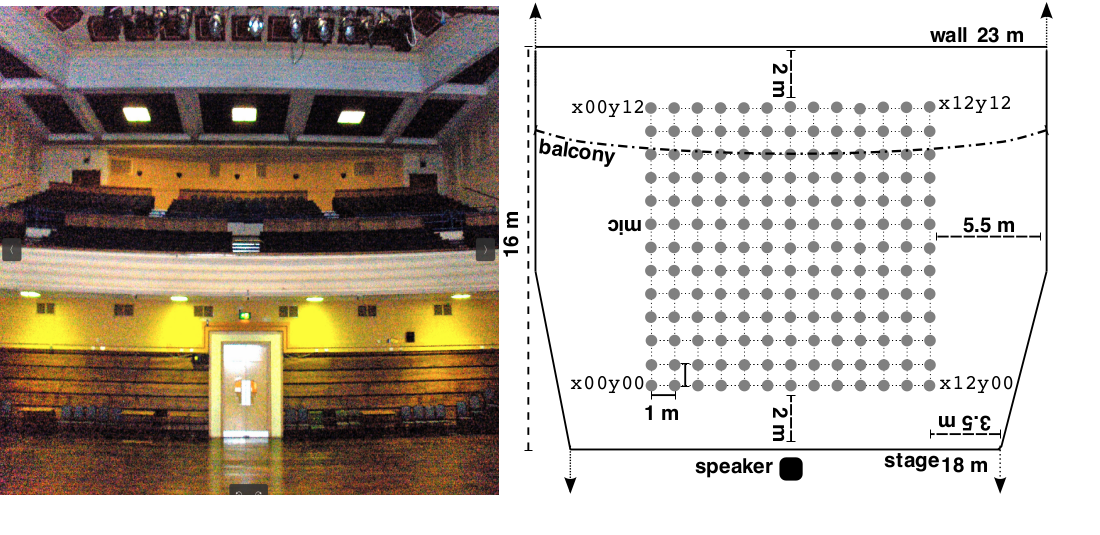
\includegraphics[scale=0.30]{greathall.png}
	\caption{Recinto greathall y esquema de medición de respuestas al impulso.}
	\label{fig:sala1}
\end{figure}

\begin{figure}[H]
	\centering{}
	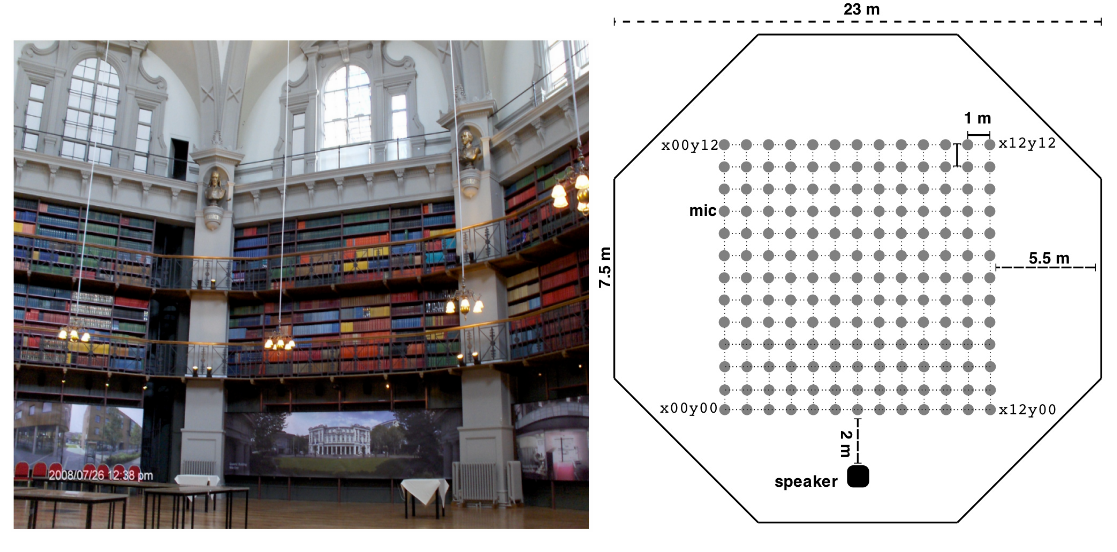
\includegraphics[scale=0.30]{octagon.png}
	\caption{Recinto octagon y esquema de medición de respuestas al impulso.}
	\label{fig:sala2}
\end{figure}

\begin{figure}[H]
	\centering{}
	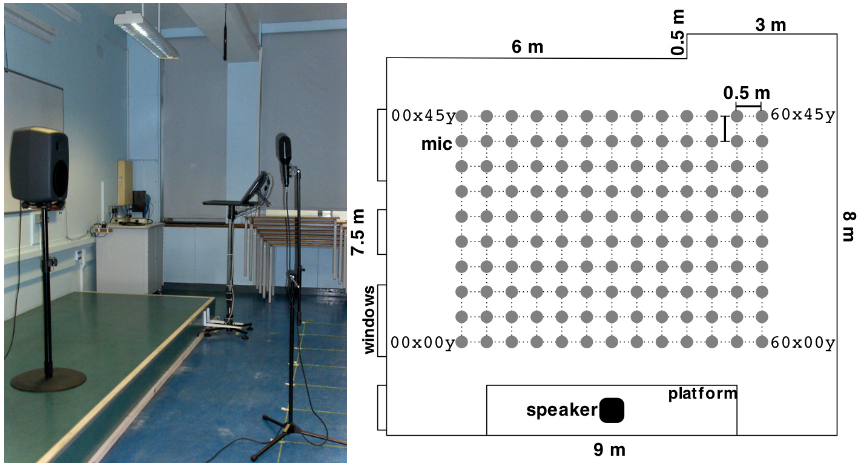
\includegraphics[scale=0.40]{classroom.png}
	\caption{Recinto classroom y esquema de medición de respuestas al impulso.}
	\label{fig:sala3}
\end{figure}



Las mediciones fueron realizadas empleando la técnica del barrido frecuencial \cite{sinesweep}, utilizando un altoparlante Genelec 8250A y un micrófono omnidireccional DPA 4006. El altoparlante mencionado es un transductor de dos vías, con un driver de 8' para frecuencias bajas-medias y un driver de 1' para frecuencias altas. En la fotografía presente en la Figura \ref{fig:sala3} se puede observar tanto el altoparlante como el micrófono dispuestos para realizar una medición.  Se miden respuestas para una única posición de fuente y varias posiciones de micrófono. Las posiciones de micrófonos se definen formando una grilla de puntos equiespaciados dentro de los recintos para realizar un mapeo uniforme, como se observa en los esquemas de medición presentados. En la Tabla \ref{table:trs_recintos} se puede ver el tiempo de reverberación por bandas para cada recinto. 


\begin{table}[H]
\centering{}
\caption{Tiempos de reverberación por bandas para cada recinto.}
\begin{adjustbox}{max width=\textwidth}
\begin{tabular}{|c|c|c|c|c|c|c|}
\hline
                    & \textbf{125 Hz} & \textbf{250 Hz} & \textbf{500 Hz} & \textbf{1000 Hz} & \textbf{2000 Hz} & \textbf{4000 Hz} \\ \hline
\textbf{Class room} & 1.80 $\pm$ 1.12 $s$ & 2.09 $\pm$ 0.12 $s$ & 2.05 $\pm$ 0.04 $s$ & 1.86 $\pm$ 0.02 $s$  & 1.99 $\pm$ 0.02 $s$  & 1.61 $\pm$ 0.01 $s$ \\ \hline
\textbf{Great Hall} & 2.19 $\pm$ 1.71 $s$ & 2.16 $\pm$ 0.29 $s$ & 2.40 $\pm$ 0.07 $s$ & 2.44 $\pm$ 0.06 $s$  & 2.30 $\pm$ 0.06 $s$  & 1.75 $\pm$ 0.06 $s$  \\ \hline
\textbf{Octagon}    & 2.40 $\pm$ 1.73 $s$ & 2.34 $\pm$ 0.11 $s$ & 2.99 $\pm$ 0.05 $s$ & 3.26 $\pm$ 0.04 $s$  & 2.91 $\pm$ 0.03 $s$  & 2.23 $\pm$ 0.03 $s$  \\ \hline
\end{tabular}
\end{adjustbox}
\label{table:trs_recintos}
\end{table}


\subsubsection{Respuestas al impulso generadas}

En cuanto a las respuestas al impulso generadas, se utilizó la librería de Python `PyRoomAcoustics' \cite{pyroom} para sintetizarlas. Esta biblioteca brinda un software de generación de respuestas al impulso basado en el método de fuente imagen  \cite{ISM}. El algoritmo está implementado en el lenguaje de programación C, permitiendo una rápida simulación de la propagación del sonido en recintos poliédricos. Los parámetros que se deben indicar a la hora de generar una respuesta al impulso son: 

\begin{itemize}
\item Dimensiones del recinto (largo, ancho y alto).
\item Posiciones de fuente y receptor, en coordenadas tridimensionales.
\item Coeficientes de absorción de las superficies.
\item Orden máximo de reflexiones a computar.
\end{itemize} 

Para generar los datos se proponen dos recintos, el primero de dimensiones $8m\: x\: 6m\: x\: 4m$ que se denominará `Recinto 1' , y el segundo de dimensiones $6m\: x\: 4m\: x\: 3.5m$ que se denominará `Recinto 2'. La cantidad de recintos generados y sus dimensiones se definen de acuerdo a los trabajos del estado del arte utilizados como referencia \cite{rir_filtinverso, FCN}.  En la Figura \ref{fig:recintos} se pueden visualizar ambos recintos generados. 

\begin{figure}[H]
\centering
\begin{subfigure}{.5\textwidth}
  \centering
  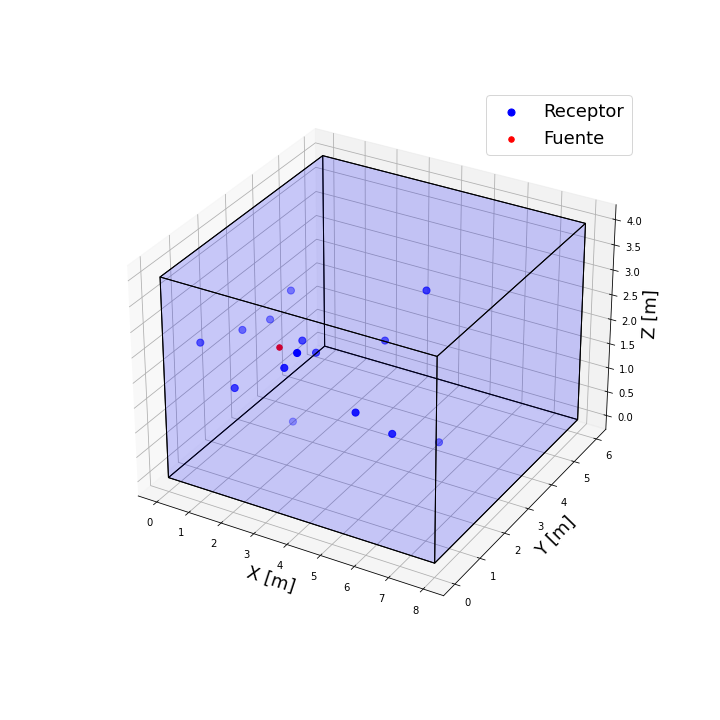
\includegraphics[scale=0.35]{room1.png}
  \caption{Recinto 1}
  \label{fig:sub1}
\end{subfigure}%
\begin{subfigure}{.5\textwidth}
  \centering
  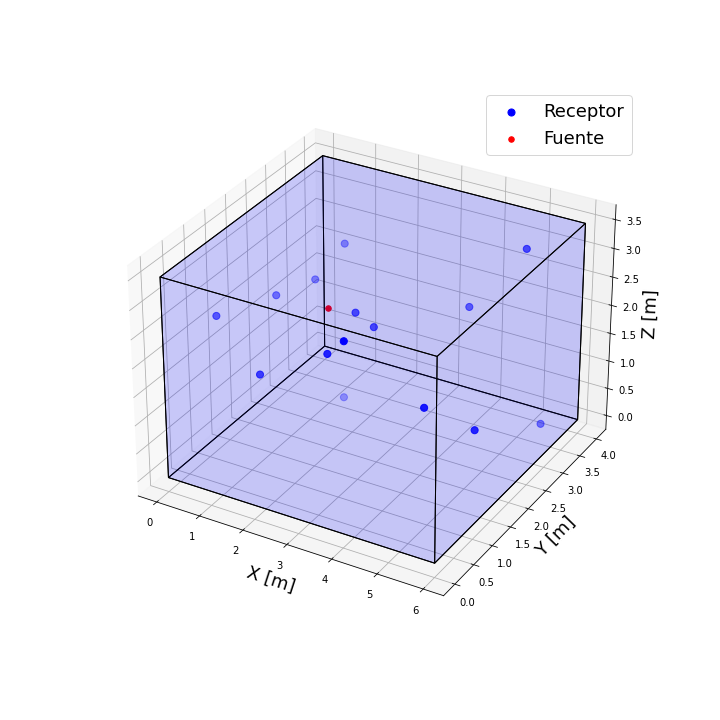
\includegraphics[scale=0.35]{room2.png}
  \caption{Recinto 2}
  \label{fig:sub2}
\end{subfigure}
\caption{Recintos y puntos receptor-fuente generados para la simulación de respuestas al impulso.}
\label{fig:recintos}
\end{figure}

Para controlar los demás parámetros que refieren a las condiciones del recinto, se subordina el orden máximo de reflexiones y los coeficientes de absorción a un tiempo de reverberación esperado. Esto es, teniendo un cierto recinto se determina un valor de tiempo de reverberación T60 inicial. Este se utiliza para estimar un valor de un coeficiente de absorción promedio mediante la ecuación de Sabine y también en base a este tiempo se determina el orden de reflexiones necesario para poder representar la reverberación. 
Por último, las posiciones de fuente y receptor se generan aleatoriamente para poder generar diferentes respuestas al impulso a partir de un mismo recinto. De esta manera, los datos que se deben determinar son las dimensiones del recinto, un tiempo de reverberación inicial y la cantidad de respuestas al impulso que se busca generar. 

Con esto, para formar el conjunto de respuestas al impulso generadas de entrenamiento se utilizó el recinto 1 para 3 tiempos de reverberación principales: $0,5 s$ como reverberación baja, $0,75 s$ como reverberación media y $1,0 s$ como reverberación alta. Partiendo de estos tiempos, se generan 30 respuestas al impulso para cada uno, variando aleatoriamente los puntos de fuente y receptor. Esto resulta en un total de 90 respuestas al impulso con tiempos de reverberación de entre aproximadamente $0.5$ segundos a $1.0$ segundos. Para generar las respuestas destinadas a evaluación se realiza el mismo procedimiento pero utilizando el recinto 2 y generando 15 respuestas por cada tiempo de reverberación, formando un total de 45 respuestas al impulso generadas. 

\subsubsection{Respuestas al impulso generadas por aumentación}

Este conjunto se obtiene a partir de respuestas al impulso reales, que generalmente son pocas y no logran una buena cobertura de los parámetros acústicos como el T60 y el DRR. Es posible, mediante técnicas de procesamiento de señales, alterar los parámetros acústicos de una respuesta al impulso, generando otras con distintas características acústicas. De esta forma, se puede ampliar considerablemente la cantidad de respuestas al impulso del conjunto de datos, a partir de alteraciones a un conjunto pequeño de respuestas al impulso reales, logrando una mejor cobertura de los parámetros acústicos de interés \cite{rir_aug}. En este trabajo, se utilizaron dos procesos para aumentar las respuestas al impulso reales: una alteración de amplitud en la parte temprana de la respuesta al impulso para controlar la relación directo-reverberado, y una alteración de envolvente de caída para controlar el tiempo de reverberación.



Para el primer proceso, a la parte correspondiente al sonido directo $h_{e}(t)$ \footnote{Comúnmente se considera que los primeros $2.5 \ ms$ corresponden al sonido directo. Esto representa una diferencia de camino de $0.85 \ m$ para una velocidad del sonido de $340 \ ms^{-1}$. Las normas de medición de respuestas al impulso establecen condiciones de posición de manera tal que la primera reflexión ocurre luego de los $2.5 \ ms$}  se le aplica una ganancia definida por un factor $\alpha$ el cual se calcula para obtener el valor de $DRR$ deseado generando una nueva señal $\tilde{h}_{e}(t)$. Para evitar generar discontinuidades durante el proceso, se aplican ventanas complementarias a la señal directa obteniendo una señal directa ventaneada y un residuo ventaneado. A partir de esto, la parte directa se puede definir según la ecuación
\ref{eqn:ventaneada}.  

\begin{equation}
\label{eqn:ventaneada}
	h_{e}(t) = \alpha w_{d}(t)h_{e}(t) + [1-w_{d}(t)]h_{e}(t)
\end{equation} 

En donde $w_{d}(t)$ corresponde a una ventana Hann de $5 ms$ de longitud. De esta manera, partiendo de esta última definición junto con la expresión del parámetro $DRR$ expresado en la ecuación \ref{eqn:DRR}, se plantea un sistema de ecuaciones a partir del cual se puede definir un valor pretendido de $DRR$ y despejar el correspondiente valor de $\alpha$. En la Figura \ref{fig:drr_aug} se puede observar una representación de una parte directa $h_{e}(t)$, las ventanas aplicadas, el efecto del factor de ganancia $\alpha$ y la nueva señal $\tilde{h}_{e}(t)$ generada. Finalmente, esta parte directa modificada se concatena con el resto de la respuesta al impulso completando así el proceso de aumentación referido a la relación directo-reverberado. Se debe tener en cuenta que para tiempos de reverberación cortos, puede ser un problema generar relaciones directo-reverberado demasiado bajas, ya que la energía de la parte tardía ya es de por si muy baja. Para esos casos, se definen valores límites para la ganancia aplicada a la parte temprana.

\begin{figure}[h]
	\centering{}
	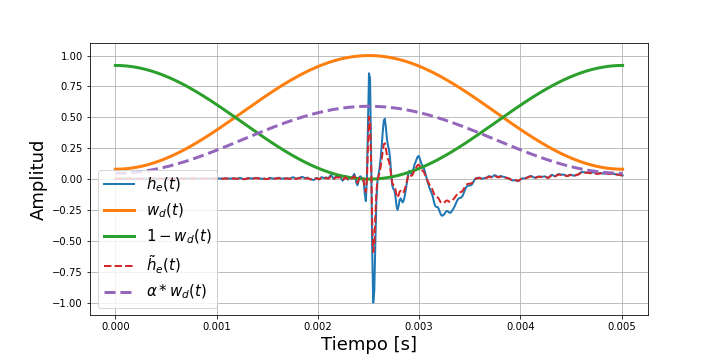
\includegraphics[scale=0.55]{drr_aug.png}
	\caption{Señales involucradas en el proceso de aumentación de DRR.}
	\label{fig:drr_aug}
\end{figure}

Luego, para la modificación del tiempo de reverberación $T_{60}$ se trabaja únicamente con la parte tardía de la respuesta al impulso. Esta puede ser modelada como ruido Gaussiano con una caída de nivel exponencial dependiente de la frecuencia, sumado a un determinado piso de ruido. Como esta pendiente de caída varía con la frecuencia, se analiza la respuesta al impulso en bandas de tercio de octava para contemplar esta dependencia frecuencial. Este modelo se expresa en la ecuación \ref{eqn:decay_exp}. 
\begin{equation}
\label{eqn:decay_exp}
	h_{m}(t) = A_{m} e^{\frac{-(t-t_{0})}{\tau_{m}}}n(t)u(t-t_{0})+\sigma_{m}n(t)
\end{equation} 
En donde $A_{m}$ es la amplitud inicial, $\tau_{m}$ es la tasa de caída, $\sigma_{m}$ es el nivel del piso de ruido, $n(t)$ es ruido Gaussiano de media cero y desvío estándar unitario, $t_{0}$ es el instante temporal en donde comienza la parte tardía de la respuesta al impulso, $m$ es el índice que refiere a una sub-banda frecuencial y $u(t)$ es un escalón unitario. En este modelo, el tiempo de reverberación $T_{60}$ se relaciona directamente con el parámetro $\tau$ según la ecuación \ref{eqn:tau60}.

\begin{equation}
\label{eqn:tau60}
	T_{60} = ln(1000)\tau T_{s}
\end{equation}

En donde $T_{s}$ es el período de muestreo. Dado este modelo, se aplican métodos de optimización no lineales para estimar el conjunto de parámetros $\left \{ \hat{A}_{m}; \hat{\tau}_{m}; \hat{\sigma}_{m} \right \}$ que mejor aproximen la envolvente de caída de la respuesta al impulso. Con estos parámetros sumados a la tasa de caída deseada $\tau_{m,d}$ calculada a partir del tiempo de reverberación deseado, se modifica la parte tardía de la respuesta al impulso inicial multiplicándola por una envolvente exponencial creciente o decreciente según corresponda como se muestra en la ecuación  \ref{eqn:aug_tr}.

\begin{equation}
\label{eqn:aug_tr}
	{h_{m}}'(t) = h_{m}(t) e^{-(t-t_{0})\frac{\hat{\tau_{m}}-\tau_{m,d}}{\hat{\tau_{m}}\tau_{m,d}}}
\end{equation}

En donde ${h_{m}}'(t)$ representa a la nueva parte tardía de la respuesta al impulso generada para obtener el tiempo de reverberación deseado. En términos generales, el proceso consiste en modificar la pendiente de caída para obtener la pendiente de caída deseada por cada banda de frecuencia. Al final, las sub-bandas generadas se suman para obtener el resultado final que contemple todo el espectro de la señal. Hasta aquí este proceso funciona satisfactoriamente cuando se generan tiempos de reverberación menores al de la respuesta al impulso inicial, es decir, siempre que se multiplica la respuesta al impulso por envolventes exponenciales decrecientes. En cambio, cuando se busca generar tiempos de reverberación mayores, la envolvente por la que se multiplica la respuesta inicial es creciente, lo que produce una amplificación de la parte tardía de la respuesta al impulso. Esto muchas veces equivale a amplificar el piso de ruido presente en la señal, lo que puede producir pendientes de caída inestables que no se corresponden con el comportamiento propio de la respuesta al impulso ya que no es información del sistema acústico sino simplemente ruido. Para evitar este efecto adverso del proceso de aumentación anteriormente propuesto se debe estimar el piso de ruido de la respuesta al impulso. Esto se realiza a través del método iterativo propuesto por Lundeby et. al. \cite{Lundeby}. Una vez estimado el piso de ruido de la señal, la respuesta final se obtiene haciendo un cross-fade en el inicio del piso de ruido entre la parte tardía generada y una cola reverberante sintética creada a partir de multiplicar ruido Gaussiano con una envolvente exponencial decreciente, utilizando los parámetros previamente calculados. Una explicación más detallada de este proceso se puede encontrar en el anexo A. 

Para realizar este proceso se determinan límites de relación directo-reverberado y tiempo de reverberación medio. La relación directo-reverberado va desde $-3 \ dB$ a $10 \ dB$ con saltos de $1 \ dB$, lo que se considera una diferencia de nivel promedio acorde a la mínima perceptible por el oído humano. Con respecto al tiempo de reverberación, se generan desde $0.1 \ s$ a $1.2 \ s$ para estar dentro del rango de las respuestas al impulso generadas, con un paso de $0.05 s$ basado en estudios previos realizados sobre la mínima diferencia perceptible entre tiempos de reverberación \cite{aug_JND}. Una vez obtenido el conjunto de respuestas al impulso aumentadas, se seleccionan aleatoriamente 135 respuestas para equiparar al número de respuestas al impulso generadas. 

\subsection[Bases de datos de señales de habla]{BASES DE DATOS DE SEÑALES DE HABLA}

Las señales de habla necesarias para formar los pares anecoico-reverberados se obtienen de la librería LibriSpeech \cite{librispeech}, la cual consiste en un conjunto de datos que reúne 100 horas de audio correspondientes a lecturas en idioma inglés. Los datos corresponden a programas tipo audiolibros. Las señales poseen bajo nivel de reverberación, y provienen de una aplicación en la cual la inteligibilidad es primordial, lo cual hace que esta base de datos sea adecuada para utilizarse en este trabajo.

\subsubsection{Pre-procesamiento de datos}

Partiendo de audios de voz y respuestas al impulso, el modelo de red neuronal propuesto requiere generar instancias de espectrogramas de magnitud correspondientes a audios anecoicos y reverberados. Para conseguir esto, se programa una cadena de procesamiento automatizada que realice esta transformación de los datos de entrada. 
En primer lugar se controla la uniformidad de frecuencias de muestreo aplicando las transformaciones de aumentación o decimado cuando sean requeridas. Se decide trabajar con una frecuencia de muestreo de $16000$ muestras por segundo, considerando que se trata con señales de voz que concentran su información por debajo de la frecuencia de Nyquist de $8000$ Hz. 
Luego, los audios de voz se convolucionan con las respuestas al impulso para formar pares de señales con y sin reverberación. El resultado de la convolución se recorta para descartar el retardo generado por la convolución, haciendo que los pares de señales sean sincrónicas. Luego, se toman ventanas rectangulares de $32640$ muestras, lo que equivale a segmentos de audio de $2,04$ segundos para la frecuencia de muestreo utilizada. Lo siguiente es aplicar la transformada de corto término de Fourier tanto a la señal limpia como a la señal convolucionada. La transformada se aplica con una ventana de $512$ muestras y un salto de $128$ muestras lo cual equivale a un solapamiento del $75\%$, el cual permite una correcta reconstrucción de la señal. El tamaño de ventana y de salto se escoge de acuerdo a los trabajos del estado del arte \cite{rir_filtinverso, FCN}. Se obtienen espectrogramas complejos, a los cuales se les calcula la magnitud, descartando la información de fase. Además, se aplica una normalización para acotar el dominio en valores que sean convenientes para el algoritmo de  aprendizaje posterior. 

Finalmente, las instancias finales de este proceso son el espectro de magnitud de la señal con reverberación (que corresponde a la variable de entrada de la red neuronal) y el espectro de magnitud de la señal sin reverberación (que corresponde a la salida deseada). Ambas instancias tienen las mismas dimensiones, que corresponden a $256$ cuadros temporales y $257$ cuadros frecuenciales (se conserva sólo la parte positiva del espectro frecuencial simétrico). Por último, se descartan los puntos correspondientes al valor máximo de frecuencia. Esto se realiza para obtener dimensiones finales de $256x256$ lo cual facilita el diseño de la red neuronal convolucional, al ser dimensiones múltiplos de $2$. Se descarta la frecuencia más alta, lo cual no compromete la representación de la señal ya que no habrá información relevante de la misma en la frecuencia de Nyquist.

Cabe destacar que debido a este preprocesamiento aplicado, a la hora de evaluar el modelo se deberán aplicar una serie de procesos previos sobre el audio a procesar. Más precisamente, se deberá segmentar el audio y obtener espectros de magnitud de la STFT respetando los mismos parámetros que en el preprocesamiento. Luego, como la salida de la red es una máscara de amplitud comprimida, se debe descomprimir esta máscara, aplicarla sobre el espectro reverberado y luego combinar el espectro de amplitud modificado resultante con la fase original de la señal para poder finalmente obtener la información de audio de salida (ya sea a través de la aplicación del algoritmo de Griffin-Lim, o bien simplemente combinando la fase del espectrograma reverberado con la magnitud dereverberada).


\subsection[Modelo propuesto]{MODELO PROPUESTO}

El modelo propuesto se basa en una arquitectura de red neuronal completamente convolucional tipo `autoencoder' inspirada en el trabajo de Ernst et. al. \cite{FCN}. En este autoencoder, la señal de salida es la señal de entrada sin reverberación. Este tipo de variantes de autoencoder se denominan denoising autoencoders \cite{DAE}, y son un patrón de diseño muy común en problemas de mejora del habla. En este trabajo, en vez de estimar directamente el espectrograma anecoico, la red estima máscaras que al ser multiplicadas con la señal reverberada de entrada, dan como resultado el espectrograma anecoico. En estudios previos, se demostró que este método da mejores resultados que estimar directamente el espectrograma anecoico \cite{mask_vs_map}. Para trabajar con espectros, las señales de entrada se transforman al dominio temporal-frecuencial a partir de la transformada de Fourier de corto término.
 
La estructura de red neuronal utilizada consiste en una U-NET con conexiones de salto, inspirada inicialmente en \cite{FCN}. Este tipo de estructura consiste en tomar mapas bidimensionales de entrada y a partir de la aplicación sucesiva de capas convolucionales con valores de salto mayor a 1, reducir la dimensionalidad del mismo e ir aumentando el número de filtros utilizados por las capas convolucionales. Un esquema básico de está estructura se puede ver en la Figura \ref{fig:unet}, en donde se puede observar que las dimensiones de las capas siguen una forma de `U', lo cual le da el nombre a estas estructuras.

\begin{figure}[H]
	\centering{}
	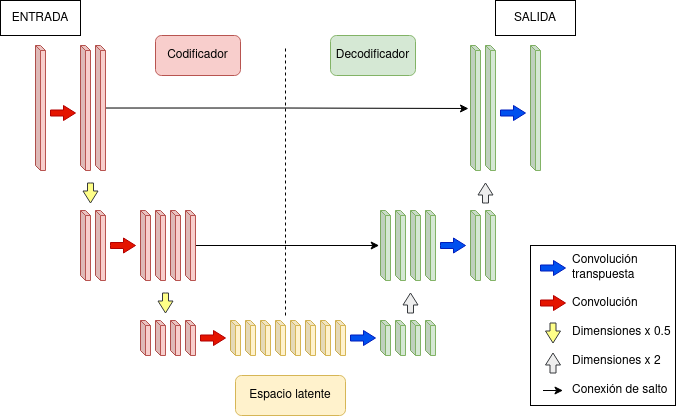
\includegraphics[scale=0.7]{unet.png}
	\caption{Esquema básico de una red tipo `U-NET' con conexiones de salto.}
	\label{fig:unet}
\end{figure}

A medida que se avanza en el modelo, las dimensiones de la imagen de entrada disminuyen y la cantidad de filtros utilizados aumentan. Esta primera etapa equivale a la función de codificación $f$ de un autoencoder. El proceso se realiza sucesivamente hasta que las dimensiones de la imagen son de 1x1, lo cual se corresponde con el espacio latente $h$. Luego, prosigue una etapa de decodificación en la cual se aplica el proceso inverso. Esto es, las dimensiones van aumentando con capas de convolución transpuesta configuradas con tamaños de saltos mayores a 1, y la cantidad de filtros utilizados va disminuyendo. Esto se repite hasta que las dimensiones del tensor sean las mismas que tenía a la entrada del codificador. Mediante este esquema de U-NET y el efecto del cuello de botella de las dimensiones, se consigue que la estimación de cada punto del espectrograma anecoico esté condicionado por todos los puntos que componen el espectrograma reverberado de entrada, y no solo por una región particular del mismo. Para poder pasar información de manera más directa desde el decodificador hacia el codificador, se implementan conexiones de salto. La conexión de salto consiste en concatenar la salida de una capa del codificador con la de una capa del decodificador. Para poder hacerlo, la dimensión de concatenación (en este caso, las dimensiones del espectrograma) deben ser las mismas. De esta manera se logran decodificaciones más precisas, y se solucionan problemas como el desvanecimiento de gradiente \cite{lagartija}. 

Una representación gráfica del modelo final implementado se puede apreciar en la Figura \ref{fig:modelo}. En cada capa se indican tres valores, donde el primero representa la dimensión temporal, el segundo la dimensión frecuencial y el tercero el número de canales (equivalente a la cantidad de filtros). En las primeras capas, las dimensiones se reducen a la mitad en cada instancia debido al uso de un desplazamiento de paso 2 en el cálculo de los filtros convolucionales. En las capas subsiguientes, las dimensiones sufren el efecto contrario hasta volver a obtener las dimensiones originales. El uso de las conexiones de salto permite que en el proceso de codificación, en el cual se reduce la dimensionalidad, no se pierda información detallada del espectrograma de entrada. Estos detalles presentes en las primeras capas del codificador, podrán ser aprovechados por las últimas capas del decodificador al existir las conexiones de salto. A su vez, el decodificador tendrá acceso a información global y general del espectrograma, la cual se encuentra codificada en el espacio latente.

\begin{figure}[H]
	\centering{}
	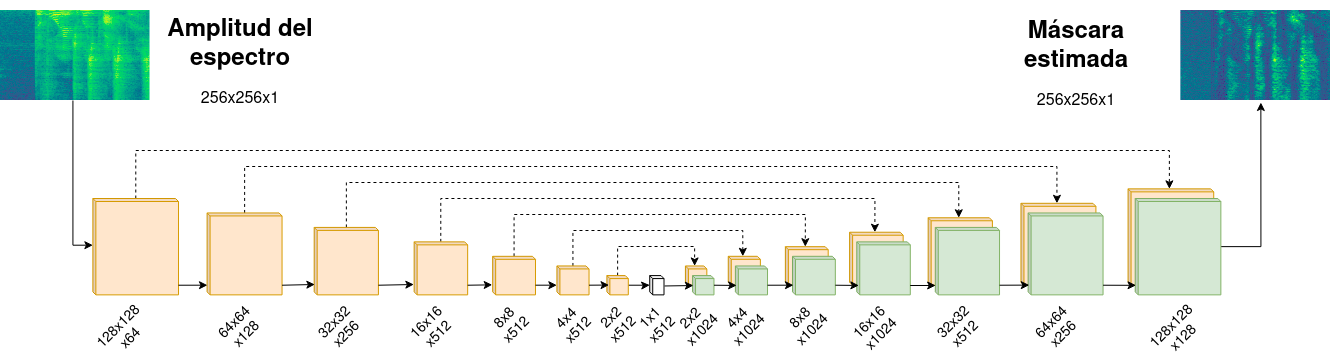
\includegraphics[scale=0.35]{modelo_red.png}
	\caption{Modelo de red neuronal convolucional implementado.}
	\label{fig:modelo}
\end{figure}

\subsection[Detalles de implementación]{DETALLES DE IMPLEMENTACIÓN}

En la arquitectura implementada, se imitaron decisiones tomadas en el trabajo de Ernst et. al. \cite{FCN}. Se utilizan activaciones tipo ReLu combinadas con LeakyReLu  de pendiente $0.2$. Se escogen estas activaciones debido a que son favorables frente al problema de desvanecimiento de gradiente, que suele ser común en redes muy profundas. Se emplean técnicas de regularización como dropout y también se realiza normalización por lotes (BatchNorm). En la Tabla \ref{table:arquitectura} se especifican las características de la arquitectura implementada. 


% Please add the following required packages to your document preamble:
% \usepackage[table,xcdraw]{xcolor}
% If you use beamer only pass "xcolor=table" option, i.e. \documentclass[xcolor=table]{beamer}
\begin{table}[H]
\caption{Especificaciones de la arquitectura implementada.}
\centering
\begin{threeparttable}
\begin{tabular}{c|
>{\columncolor[HTML]{FFFC9E}}c 
>{\columncolor[HTML]{FFFC9E}}c 
>{\columncolor[HTML]{FFFC9E}}c |
>{\columncolor[HTML]{9AFF99}}c 
>{\columncolor[HTML]{9AFF99}}c 
>{\columncolor[HTML]{9AFF99}}c |}
\cline{2-7}
                                                            & \multicolumn{3}{c|}{\cellcolor[HTML]{FFFC9E}\textbf{ENCODER}}                                                             & \multicolumn{3}{c|}{\cellcolor[HTML]{9AFF99}\textbf{DECODER}}                                                             \\ \hline
\multicolumn{1}{|c|}{\cellcolor[HTML]{ECF4FF}\textbf{Capa}} & \textbf{Filtros} & \textbf{Activación} & \textbf{\begin{tabular}[c]{@{}c@{}}Regularización/\\ Normalización\end{tabular}} & \textbf{Filtros} & \textbf{Activación} & \textbf{\begin{tabular}[c]{@{}c@{}}Regularización/\\ Normalización\end{tabular}} \\ \hline
\multicolumn{1}{|c|}{\cellcolor[HTML]{ECF4FF}1}             & 64               & LeakyReLu           & -                                                                                & 512              & ReLu                & BatchNorm-Dropout                                                                \\
\multicolumn{1}{|c|}{\cellcolor[HTML]{ECF4FF}2}             & 128              & LeakyReLu           & BatchNorm                                                                        & 512              & ReLu                & BatchNorm-Dropout                                                                \\
\multicolumn{1}{|c|}{\cellcolor[HTML]{ECF4FF}3}             & 256              & LeakyReLu           & BatchNorm                                                                        & 512              & ReLu                & BatchNorm-Dropout                                                                \\
\multicolumn{1}{|c|}{\cellcolor[HTML]{ECF4FF}4}             & 512              & LeakyReLu           & BatchNorm                                                                        & 512              & ReLu                & BatchNorm                                                                        \\
\multicolumn{1}{|c|}{\cellcolor[HTML]{ECF4FF}5}             & 512              & LeakyReLu           & BatchNorm                                                                        & 256              & ReLu                & BatchNorm                                                                        \\
\multicolumn{1}{|c|}{\cellcolor[HTML]{ECF4FF}6}             & 512              & LeakyReLu           & BatchNorm                                                                        & 128              & ReLu                & BatchNorm                                                                        \\
\multicolumn{1}{|c|}{\cellcolor[HTML]{ECF4FF}7}             & 512              & LeakyReLu           & BatchNorm                                                                        & 64               & ReLu                & BatchNorm                                                                        \\
\multicolumn{1}{|c|}{\cellcolor[HTML]{ECF4FF}8}             & 512              & ReLu                & BatchNorm                                                                        & 1                & ReLu \tnote{1}                & BatchNorm                                                                        \\ \hline
\end{tabular}
	\begin{tablenotes}
    	\item[1] Se cambia a ReLu limitada en 1 a la hora de hacer predicciones.
	\end{tablenotes}
\end{threeparttable}
\label{table:arquitectura}
\end{table}


Las capas que componen el codificador son convolucionales, y las que componen el decodificador son capas deconvolutivas o de convolución transpuesta. Las capas de convolución transpuesta pueden generar artefactos indeseados en los mapas de características \cite{checkerboard}.  Una manera de solucionar este efecto es asegurándose de que los campos receptivos sean múltiplos enteros del tamaño de salto utilizado \cite{check1}. Sin embargo, aun teniendo esto en consideración, las capas de convolución transpuesta pueden seguir generando artefactos. Entonces, en lugar de utilizar capas de convolución transpuesta se opta por implementar una combinación de dos capas consecutivas: en primer lugar una capa que aumente las dimensiones del espectrograma generando nuevos puntos a partir de una interpolación entre los valores más cercanos, y luego una capa convolucional. De esta manera se logra aumentar la dimensionalidad de la entrada y utilizar una operación de convolución sin generar la aparición de artefactos indeseados \cite{check2}. 
En todas las capas tanto del codificador como del decodificador se utiliza un tamaño de filtro de $6x6$ y un tamaño de salto igual a $2$. 

%%
Finalmente, la función de costo utilizada para evaluar las predicciones realizadas por el modelo frente a las máscaras ideales en la salida es el error cuadrático medio (MSE), el cual se expresa en la ecuación \ref{eqn:mse}. Para la optimización se utilizó el algoritmo de estimación adaptativa de momento (ADAM) \cite{adam} con un valor de tasa de aprendizaje de $0,001$. 

\begin{equation}
\label{eqn:mse}
	L_{MSE} = \sum_{i=1}^{N-1}(M_{i}(t,f) - \hat{M}_{i}(t,f))^{2}
\end{equation}

La arquitectura de red neuronal se implementó utilizando el lenguaje de programación Python (versión 3.7), particularmente haciendo uso de la biblioteca Tensorflow\footnote{Página oficial de Tensorflow: \url{https://www.tensorflow.org/}}, la cual permite el desarrollo y entrenamiento de modelos de aprendizaje por máquina.  


\subsection[Evaluación del modelo]{EVALUACIÓN DEL MODELO}
En este trabajo se evalúa el impacto que provoca la aumentación, simulación y ordenamiento de datos en el desempeño del modelo.
Particularmente, se analiza el aporte de realizar aumentación de respuestas al impulso reales, y de sintetizar nuevas respuestas al impulso. También se evalúa el efecto del ordenamiento de los datos durante el entrenamiento de la red.

\subsubsection{Combinaciones de bases de datos}
En primer lugar, como se cuenta con respuestas al impulso reales, generadas  y aumentadas, se prueban combinaciones de estos datos a la hora de formar los diferentes conjuntos de entrenamiento y evaluación. Es decir, se entrena el modelo utilizando un determinado conjunto, y luego se evalúa su funcionamiento sobre el total de los conjuntos. Esto resulta en 3 pruebas, en donde los conjuntos de entrenamiento y evaluación quedan determinados según la Tabla \ref{tab:pruebas}. Cabe aclarar que los conjuntos utilizados para entrenamiento no son los mismos que los utilizados para la evaluación en cada prueba. Es decir, cuando por ejemplo se entrena con reales y se evalúa sobre reales, en cada proceso se utilizan conjuntos de datos distintos.


\begin{table}[H]
\caption{Configuración del primer conjunto de pruebas.}
\centering
\begin{tabular}{|c|c|c|c|}
\hline
                          & \textbf{Prueba 1}                                                       & \textbf{Prueba 2}                                                       & \textbf{Prueba 3}                                                       \\ \hline
Conjunto de entrenamiento & Reales                                                                  & Generadas                                                               & Aumentadas                                                              \\ \hline
Conjuntos de evaluación   & \begin{tabular}[c]{@{}c@{}}Reales\\ Generadas\\ Aumentadas\end{tabular} & \begin{tabular}[c]{@{}c@{}}Reales\\ Generadas\\ Aumentadas\end{tabular} & \begin{tabular}[c]{@{}c@{}}Reales\\ Generadas\\ Aumentadas\end{tabular} \\ \hline
\end{tabular}
\label{tab:pruebas}
\end{table}

Luego, se evalúa el desempeño del modelo propuesto al utilizar combinaciones de conjuntos en la etapa de entrenamiento. Como el objetivo principal es contar con una mayor cantidad y variedad de respuestas al impulso, en vez de solo utilizar respuestas grabadas, las combinaciones propuestas consisten en combinar las respuestas reales con las generadas y aumentadas como se indica en la Tabla \ref{tab:pruebas_combinadas}. 

\begin{table}[H]
\caption{Configuración del segundo conjunto de pruebas.}
\centering
\begin{tabular}{|c|c|c|c|}
\hline
                          & \textbf{Prueba 1}                                                       & \textbf{Prueba 2}                                                       & \textbf{Prueba 3}                                                                   \\ \hline
Conjunto de entrenamiento & \begin{tabular}[c]{@{}c@{}}Reales \\ + \\ Aumentadas\end{tabular}       & \begin{tabular}[c]{@{}c@{}}Reales\\  + \\ Generadas\end{tabular}        & \begin{tabular}[c]{@{}c@{}}Reales \\ + \\ Aumentadas \\ + \\ Generadas\end{tabular} \\ \hline
Conjuntos de evaluación   & \begin{tabular}[c]{@{}c@{}}Reales\\ Generadas\\ Aumentadas\end{tabular} & \begin{tabular}[c]{@{}c@{}}Reales\\ Generadas\\ Aumentadas\end{tabular} & \begin{tabular}[c]{@{}c@{}}Reales\\ Generadas\\ Aumentadas\end{tabular}             \\ \hline
\end{tabular}
\label{tab:pruebas_combinadas}
\end{table}

\subsubsection{Ordenamiento de los datos durante el entrenamiento}

Por otro lado, se evalúa la influencia del orden con el que las instancias de entrenamiento se le presentan a la red. Normalmente, durante el entrenamiento de una red neuronal, los datos se ordenan de forma aleatoria. Sin embargo, diversos trabajos \cite{cv, cl1, cl2}, demuestran que ordenar los datos de forma creciente en dificultad es beneficioso y lleva a un mejor desempeño de los modelos. Esta técnica se denomina aprendizaje por currículum, y para este trabajo, el criterio que se utilizó para medir la dificultad es que a mayor tiempo de reverberación (TR), más difícil es dereverberar una señal. En consecuencia, se evaluó el modelo entrenado con los datos en un orden creciente de TR (currículum), y para evaluar la efectividad del método, se comparó su desempeño con entrenar el modelo con un orden decreciente de TR (anti-currículum), y con un orden aleatorio.

Para esta evaluación del orden de los datos en el entrenamiento, es necesario generar un conjunto de datos anecoicos-reverberados de manera controlada, asegurando una distribución homogénea de los tiempos de reverberación presentes en el conjunto final. Para conseguir esto se decide conformar el conjunto de datos a partir de respuestas al impulso aumentadas, ya que estas se pueden generar controlando paramétricamente el TR medio y la DRR. Se busca cubrir el rango de tiempo de reverberación medio desde $0.1 \ s$ hasta $3.5 \ s$ con variaciones de entre $-10 \ dB$ a $10 \ dB$ de relación directo-reverberado. 
